\section*{Ex.\ 3.3 \quad (5 pts) --- servicing a fault when every frame is in use}

No frame is free, so the page cannot be read in until the OS takes one away. The
fault handler must:

\begin{enumerate}[itemsep=1pt,topsep=3pt]
  \item \textbf{Choose a victim frame}, using a replacement policy (Ex.\ 3.8).
  \item \textbf{Clean the victim if it is dirty.} Test its modified bit $M$. If
        $M=1$ the frame no longer matches its copy on disk and must be written to
        the swap area first; if $M=0$ that copy is still valid and the frame can be
        taken at once.
  \item \textbf{Break the old mapping.} Mark the victim's page-table entry
        not-present in its owner's page table \emph{and} invalidate the matching TLB
        entry, or a stale translation will keep reaching a frame that now holds a
        different page.
  \item \textbf{Read the wanted page} from disk into the freed frame. The faulting
        process blocks for the duration and the CPU goes to another process.
  \item \textbf{Install the new mapping}: frame number into the faulting entry,
        present bit set, $R$ and $M$ cleared, protection bits set.
  \item \textbf{Back up and restart the faulting instruction} (Ex.\ 3.7).
\end{enumerate}

Steps 2 and 4 are each a disk access, so a fault that must clean its victim costs
about twice one that need not; systems therefore keep a pool of pre-cleaned free
frames (Ex.\ 3.6) to move the write-back off the fault path.

\section*{Ex.\ 3.4 \quad (5 pts) --- why NFU over LRU}

Cost, and often availability. Exact LRU has to know the order of \emph{every}
reference, and a reference that hits a valid page-table entry is resolved by the MMU
without the OS ever seeing it. True LRU must therefore be built in hardware: a
counter or clock value written into the entry on every access, with a scan of all
frames at eviction time to find the minimum; or a list moved-to-front on every
access; or an $n \times n$ matrix of bits updated per reference. Such specialised hardware is rare, so on most machines exact LRU is unavailable at any price, and
where it exists it taxes every memory access.

NFU, as defined in Ex.\ 3.8, needs only the reference bit that essentially every MMU
already maintains for free. Its work happens once per clock tick --- add $R$ to the
page's counter, clear $R$ --- which is $O(\text{frames})$ per tick instead of $O(1)$
per reference, and it is ordinary software that ports to any MMU with an $R$ bit.

What is given up: NFU ranks pages by how \emph{often} they were used over their whole
lifetime rather than how \emph{recently}, and cannot order two references in the same
tick. It is the right choice when LRU's hardware is missing or its per-reference cost
unaffordable.

\section*{Ex.\ 3.5 \quad (5 pts) --- why NFU with aging over NFU or LRU}

\textbf{Over plain NFU.} NFU's counter is a lifetime total that is never reduced, so
the algorithm never forgets. A page referenced heavily during start-up keeps a large
count permanently and is protected long after it has gone cold, while a page that has
only just become busy has a small count and is evicted in its place. Pages that were
all once busy accumulate large, indistinguishable counts with no basis for choosing
between them.

Aging keeps the per-tick sampling but changes the arithmetic: each tick the counter is
shifted right one bit and $R$ is inserted at the \emph{high-order} end. A reference's
contribution therefore halves every tick, so the counter is dominated by recent
history and the position of its highest set bit says how long ago the page was last
touched. The smallest counter is now approximately the least recently used page:
recency rather than lifetime frequency.

\textbf{Over LRU.} The cost argument of Ex.\ 3.4 is unchanged: a reference bit, one
shift and one OR per page per tick, all in software.

\textbf{What it still cannot do.} The counter has finite width, typically 8 bits, so
pages untouched for more than 8 ticks all read zero and cannot be separated, and two
references within one tick look like one. Aging approximates LRU; it does not
implement it.

\section*{Ex.\ 3.6 \quad (5 pts) --- what the two-handed clock is for}

Its purpose is to separate \emph{clearing} reference bits from \emph{evicting} pages,
so that the rate of each can be set independently.

With one hand the same pointer does both jobs, so how fast it turns is set entirely by
the eviction rate. On a machine with a lot of memory a revolution takes so long that by
the time the hand returns nearly every page has been touched again; it finds $R=1$
almost everywhere, clears bits and sweeps on, and the page it finally takes is chosen
by position in the frame list rather than by recent use --- FIFO behaviour. Driving it
faster fails the other way, leaving pages too little time to set $R$ so that nearly all
of them look unreferenced.

Two hands fix the window. The front hand clears $R$; the back hand, a fixed distance
behind, releases any page whose $R$ is still clear, so it went unreferenced while the
gap was traversed. The gap is the test interval, a tunable parameter rather than a side
effect of memory size and load.

\begin{center}
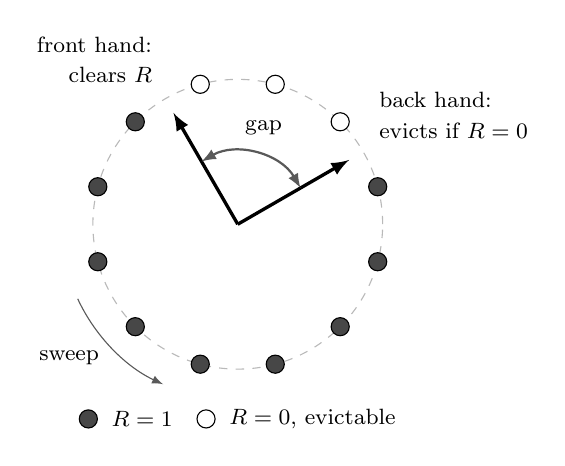
\begin{tikzpicture}[scale=1.15,>=latex]
  % ring of page frames
  \draw[gray!55,dashed] (0,0) circle (1.6);
  \foreach \a in {45,75,105}
    \draw[fill=white,draw=black] (\a:1.6) circle (0.1);
  \foreach \a in {135,165,195,225,255,285,315,345,15}
    \draw[fill=black!72,draw=black] (\a:1.6) circle (0.1);
  % the two hands
  \draw[very thick,->] (0,0) -- (120:1.42);
  \draw[very thick,->] (0,0) -- (30:1.42);
  % gap between the hands
  \draw[<->,thick,black!65] (30:0.8) arc (30:120:0.8);
  \node at (75:1.1) {\footnotesize gap};
  % hand labels
  \node[anchor=south east,align=right] at (120:1.68)
    {\footnotesize front hand:\\[-1pt]\footnotesize clears $R$};
  \node[anchor=south west,align=left] at (30:1.68)
    {\footnotesize back hand:\\[-1pt]\footnotesize evicts if $R=0$};
  % sweep direction, outside the ring at lower left
  \draw[->,black!65] (205:1.95) arc (205:245:1.95);
  \node[anchor=east] at (226:2.05) {\footnotesize sweep};
  % legend, clear of the ring
  \draw[fill=black!72,draw=black] (-1.65,-2.15) circle (0.1);
  \node[anchor=west] at (-1.5,-2.15) {\footnotesize $R=1$};
  \draw[fill=white,draw=black] (-0.35,-2.15) circle (0.1);
  \node[anchor=west] at (-0.2,-2.15) {\footnotesize $R=0$, evictable};
\end{tikzpicture}
\end{center}

BSD's pageout daemon uses this to keep a free-frame pool: woken periodically, it sweeps
only as far as needed to restore \texttt{lotsfree} free frames, so a fault normally
finds a clean frame waiting instead of paying for a scan and a write-back (Ex.\ 3.3).

\section*{Ex.\ 3.7 \quad (10 pts) --- backing up the instruction after a page fault}

\textbf{Which instruction.} The one that was executing when the fault was taken ---
the faulting instruction itself. It must be re-executed from its first byte, so the PC
saved by the trap has to be backed up to the start of that instruction. Not the one
before it, and not resumed from the middle.

\textbf{Why it has to be backed up.} \emph{The memory access never happened.} The instruction was abandoned at the operand
reference that missed, so its effect was never produced; returning to the following
instruction would silently skip a load or a store. Paging must be invisible to the
program, and the only way to make the access occur is to execute the instruction again.

\emph{The saved PC need not point at the start of it.} On a variable-length CISC
encoding the PC advances as the instruction is decoded, so when the fault is taken it
may already be past the opcode and some operand bytes; on the 68000 it points just
after the part that faulted. The handler cannot recover the start by scanning
backwards, since with variable-length encodings there is no telling where the preceding
instruction began, so the hardware must supply the address.

\emph{Side effects may already be committed.} Auto-increment and auto-decrement modes
update their index register as a side effect, and a block move copies as it goes. A
fault partway through leaves registers already stepped and part of the block written.
Re-executing from the start applies those updates twice; resuming skips the transfer.
Either way the program gets a wrong answer unless the partial effects are undone first.

So machines either record enough internal state for microcode or the handler to unwind
what was done and recompute the starting address, or define their instructions to be
restartable: every fault detected before any register is altered, with the faulting
address kept in a dedicated register, as RISC machines do.

\section*{Ex.\ 3.8 \quad (10 pts, 2 pts each) --- five page replacement algorithms}

\textbf{FIFO.} Keep the resident pages on a queue in load order; evict the one at the
head, which has been resident longest, and append the arrival at the tail. One pointer,
no hardware support, and no usage information at all --- so a page in constant use is
discarded simply for being old. FIFO is not a stack algorithm and can show Belady's
anomaly, where giving it more frames \emph{increases} the number of faults.

\textbf{FILO (first-in last-out).} The complement, as the name is used here: the
resident pages form a stack and the victim is the most recently loaded one, so arrivals
keep reusing the same frame. As cheap as FIFO and far worse, because the newest page is
precisely the one the current locality has just demanded; it is thrown out at once while
the rest of memory never turns over.

\textbf{NRU (not recently used).} Sort pages by their $(R,M)$ bits into four classes,
numbered 0 to 3 for $(0,0)$, $(0,1)$, $(1,0)$, $(1,1)$, and evict an arbitrary page
from the lowest-numbered non-empty class. $R$ is cleared on every clock tick, so it
means ``referenced since the last tick'', while $M$ is left alone. Cheap, and it
prefers a clean unreferenced page, which needs no write-back.

\textbf{LRU.} Evict the page that has gone unreferenced longest, on the assumption that
recent use predicts imminent use. Exact implementation needs work on every reference: a
timestamp written into the page-table entry at each access, a list reordered at each
access, or an $n \times n$ matrix of bits. LRU is a stack algorithm and so is immune to
Belady's anomaly; its cost is why the approximations exist.

\textbf{NFU (not frequently used).} One software counter per page. At each clock tick
the OS adds that page's $R$ bit to its counter and clears $R$, and the page with the
smallest counter is evicted. It needs only the reference bit, but it measures frequency
over a page's entire lifetime and never forgets, so a page that was busy early keeps a
high score after going cold --- the flaw that aging removes (Ex.\ 3.5).
